


\chapter{Introducing time}




\section{A new multi-structure}

In addition to the multi-structures of multi-points, multi-paths, multi-surfaces, and multi-volumes, utilizing time now introduces a new multi-structure: the {\bf multi-event}. 

An ``event" is the space-time equivalent of a point. An event is characterized by not just a position, but also by a time. In a similar manner to how copies of the same point occupying the same position creates points with different weights, multiple events occurring at the same position and time create events with different ``weights". Events with a positive weight will be commonly referred to as ``creation events", while events with a negative weight will commonly be referred to as ``destruction events". In the image below, events with a positive weight are indicated using orange dots with a ``." in the center, while events with a negative weight are indicated using purple dots with a ``X" in the center. 

\begin{center}
\begin{tabular}{cc}
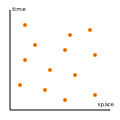
\includegraphics[width = 0.5\textwidth]{Time/multi-event_simple} & 
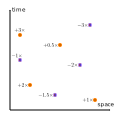
\includegraphics[width = 0.5\textwidth]{Time/multi-event_multiplicity}
\end{tabular}
\end{center}




\section{How multi-structures change with time}

This section will detail the manner in which the previously introduced multi-structures, multi-points; multi-paths; multi-surfaces; and multi-volumes, evolve with time:


\subsection{Moving points}

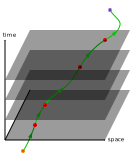
\includegraphics[width = 0.5\textwidth]{Time/world_lines}

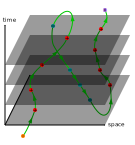
\includegraphics[width = 0.5\textwidth]{Time/world_lines_2}

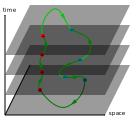
\includegraphics[width = 0.5\textwidth]{Time/world_lines_3}

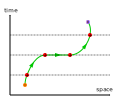
\includegraphics[width = 0.5\textwidth]{Time/infinitely_fast_point}




\section{New intersections}  


\begin{thm}
Given any multi-paths \(\mathbf{J}_1\) and \(\mathbf{J}_2\), it is the case that:
\[\mathbf{J}_1 \otimes \mathbf{J}_2 = \mathbf{J}_2 \otimes \mathbf{J}_1\]
\end{thm}


\begin{thm}
Given multi-path \(\mathbf{J}\) and multi-surface \(\mathbf{F}\), it is the case that: 
\[(\mathbf{J} \bullet \mathbf{F}) \odot \mathbf{F} = 0\]
\end{thm}


A summary of the notations used for various intersections is given below:

\vspace{5mm}

\begin{tabular}{|c||c|c|c|c|c|}
\hline
Intersections & event \(\xi_2\) & point \(\rho_2\) & path \(\mathbf{J}_2\) & surface \(\mathbf{F}_2\) & volume \(U_2\) \\
\hline
\hline
event \(\xi_1\) & 
N/A & 
N/A & 
N/A & 
N/A & 
\(\xi_1 \cdot U_2\) \\
\hline
point \(\rho_1\) & 
N/A & 
N/A & 
N/A & 
event \(\rho_1 \odot \mathbf{F}_2\) & 
point \(\rho_1 \cdot U_2\) \\ 
\hline
path \(\mathbf{J}_1\) & 
N/A & 
N/A & 
event \(\mathbf{J}_1 \otimes \mathbf{J}_2\) & 
point \(\mathbf{J}_1 \bullet \mathbf{F}_2\) & 
path \(\mathbf{J}_1 \cdot U_2\) \\ 
\hline
surface \(\mathbf{F}_1\) & 
N/A & 
event \(\mathbf{F}_1 \odot \rho_2\) &
point \(\mathbf{F}_1 \bullet \mathbf{J}_2\) & 
path \(\mathbf{F}_1 \times \mathbf{F}_2\) & 
surface \(\mathbf{F}_1 \cdot U_2\) \\ 
\hline
volume \(U_1\) & 
event \(U_1 \cdot \xi_2\) & 
point \(U_1 \cdot \rho_2\) & 
path \(U_1 \cdot \mathbf{J}_2\) & 
surface \(U_1 \cdot \mathbf{F}_2\) & 
volume \(U_1 \cdot U_2\) \\
\hline
\end{tabular}

\vspace{5mm}

%In \red{red} is indicated the ``dimensionality" of the multi-structure. Points have \(0\) dimensions; paths have \(1\) dimension; surfaces have \(2\) dimensions; and volumes have \(3\) dimensions. The number of dimensions of the intersection is the sum of the dimensions minus \(3\). When the resultant number of dimensions is less than \(0\), the intersection does not exist.



\section*{Event totals}




\section*{Creation/destruction events} 



A summary of the notations used for the different boundaries is given below. In addition, we have observed that the boundaries have no boundaries themselves.

\begin{center}
\begin{tabular}{|c||c|c|c|}
\hline
multi-structure & boundary & orientation & no boundary of the boundary property \\
\hline
\hline
event \(\xi\) & 
N/A & 
N/A & 
N/A \\ 
\hline 
point \(\rho\) &
event \(\nabla \odot \rho\) &
\parbox{0.25\textwidth}{
positive creation, negative destruction
} & 
\(\int (\nabla \odot \rho) = 0\) \\ 
\hline 
path \(\mathbf{J}\) & 
point \(\nabla \bullet \mathbf{J}\) & 
positive start, negative end &
\(\nabla \odot (\nabla \bullet \mathbf{J}) = 0\) \\
\hline
surface \(\mathbf{F}\) & 
path \(\nabla \times \mathbf{F}\) & 
counterclockwise &
\(\nabla \bullet (\nabla \times \mathbf{F}) = 0\) \\
\hline
volume \(U\) & 
surface \(\nabla U\) & 
inwards-oriented & 
\(\nabla \times (\nabla U) = 0\) \\
\hline
\end{tabular}
\end{center}

%In \red{red} is indicated the ``dimensionality" of the multi-structure. Points have \(0\) dimensions; paths have \(1\) dimension; surfaces have \(2\) dimensions; and volumes have \(3\) dimensions. The number of dimensions of the boundary is the number of dimensions minus \(1\). When the resultant number of dimensions is less than \(0\), the boundary does not exist.



\subsection*{Balanced multi-points redefined}


\section*{Event totals}





